\section{Технический проект}
\subsection{Общая характеристика организации решения задачи}

Задача заключается в разработке интеллектуальной системы для диагностики заболеваний сельскохозяйственных растений, с фокусом на томатах. Система реализована как веб-приложение, которое анализирует изображения листьев, ищет признаки заболеваний с помощью нейросетевой модели YOLOv11 и предоставляет рекомендации по лечению и профилактике. Приложение поможет агрономам и дачникам быстро выявлять болезни растений и принимать меры для сохранения урожая.

\subsection{Обоснование выбора технологии проектирования}

Для создания приложения выбраны технологии, которые обеспечивают высокую производительность, удобство для пользователей и простоту интеграции с моделью машинного обучения.

\subsubsection{Язык программирования Python}

Python -- высокоуровневый язык программирования с динамической типизацией. Его интерпретатор позволяет запускать код на различных платформах, включая Windows, macOS и Linux, без необходимости компиляции. Официальная документация поддерживает разные подходы к программированию, включая процедурный, объектно-ориентированный и функциональный стили, что даёт разработчикам гибкость\cite{python2} \cite{python3}. 

В 2025 году Python остаётся одним из самых популярных языков благодаря своему простому синтаксису и большому количеству  библиотек, которые и позволяют создавать на нём веб-приложения и модели ИИ \cite{python4}\cite{python1}.

\subsubsection{Google Colab}

Google Colaboratory (или просто Colab) -- это бесплатная облачная среда от компании Google для запуска Python-кода. Она позволяет работать с блокнотами Jupyter прямо в браузере, не требуя установки дополнительных программ на компьютер пользователя \cite{colab1}.

Одним из главных преимуществ Colab является доступ к вычислительным ресурсам GPU и TPU, что делает его особенно полезным для обучения и тестирования моделей машинного обучения и нейросетей.

\subsubsection{Фреймворк PyTorch}

PyTorch -- это инструмент, созданный для работы с нейронными сетями на Python. Он используется разработчиками, когда нужно быстро протестировать идею и собрать прототип, особенно в проектах, связанных с машинным обучением. Его ценят за гибкость, читаемость кода и большое количество готовых решений.

Открытый исходный код PyTorch позволяет любому разработчику внести изменения или адаптировать его под собственные задачи. Благодаря этому вокруг проекта сформировалось большое и активное сообщество. Постоянно появляются новые библиотеки, расширения и обучающие материалы, которые делают работу с фреймворком ещё проще \cite{yolo6}.

Среди особенностей -- поддержка как классических, так и продвинутых архитектур нейросетей. Встроенные модули позволяют обрабатывать данные, визуализировать результаты и отслеживать, как ведёт себя модель во время обучения.

Благодаря всему этому PyTorch активно применяется в разных сферах.

\subsubsection{YOLO 11}

YOLOv11 -- это одна из последних разработок в серии алгоритмов для распознавания объектов на изображениях. Эту версию представила команда Ultralytics. Данная модель стала логичным продолжением предыдущих модификаций YOLO, сохранив при этом основной подход: находить и определять объекты за один проход по изображению \cite{yolo8}.

Главное, за что ценят YOLO -- это скорость и точность. Она справляется с обработкой видео и изображений практически в реальном времени. Такая производительность достигается благодаря улучшенной архитектуре сверточной нейросети и доработанному механизму обучения. Разработчики также внедрили более точные методы предобработки данных, что заметно повысило стабильность работы модели \cite{yolo2}. 

На изображении ~\ref{graf:image} представлены результаты сравнения 11-ой версии с предшествующими ей. 

\begin{figure}[H]
	\centering
	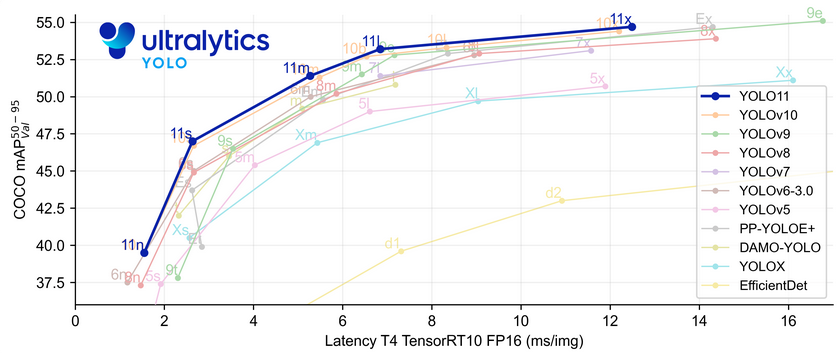
\includegraphics[width=1\linewidth]{garfYolo.png}
	\caption{График сравнения версий YOLO}
	\label{graf:image}
\end{figure}

\subsubsection{Фреймворк Flask}

Flask -- это легковесный веб-фреймворк на языке Python, который часто используют для разработки простых и понятных веб-приложений. Он не навязывает структуру проекта, поэтому подойдёт как новичкам, так и разработчикам, которым нужен контроль над архитектурой \cite{flask1}.

В отличие от более тяжёлых решений, Flask не включает в себя избыточных модулей. Вместо этого он предлагает только базовые инструменты -- маршрутизацию, работу с запросами и шаблонизатор \cite{flask2}.

Для разработки веб-интерфейса системы распознавания заболеваний растений Flask подойдёт особенно хорошо. Он позволяет быстро реализовать обработку изображений, вывод результатов и взаимодействие с нейросетью. Благодаря простому синтаксису и большому количеству обучающей информации, с реализацией приложений не возникает серьёзных трудностей, даже при ограниченном опыте в веб-программировании \cite{flask4}.

Фреймворк хорошо работает на любых операционных системах и легко разворачивается как на локальной машине, так и на сервере. Это делает Flask удобным выбором для небольших и средних проектов.

\subsubsection{PostgreSQL}

PostgreSQL -- это СУБД с открытым исходным кодом. Она известна своей стабильностью, надёжностью и соответствием стандартам SQL \cite{postgres1}.

PostgreSQL активно используется как в небольших проектах, так и в крупных корпоративных системах. Среди её ключевых особенностей -- поддержка сложных запросов, транзакций, расширяемость и работа с JSON-данными. Это делает её удобной для современных веб-приложений \cite{postgres2}.

В этой работе PostgreSQL используется для хранения данных о болезнях растений, их признаках и рекомендациях по лечению.

\subsection{Архитектура программной системы}

На рисунке \ref{comp:image} показана архитектура программной системы.
 
 \begin{figure}[ht]
 	\center{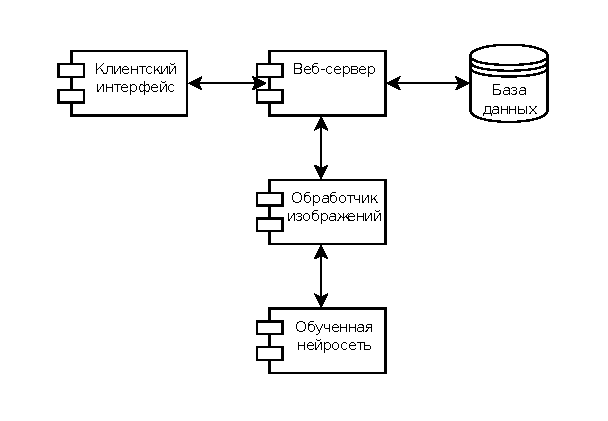
\includegraphics[width=1\linewidth]{Компоненты.eps}}
 	\caption{Диаграмма компонентов}
 	\label{comp:image}
 \end{figure}
 
 Диаграмма показывает, как устроено веб-приложение для диагностики заболеваний томатов. Она представлена в виде схемы с пятью основными блоками, соединёнными стрелками. Они указывают, как данные передаются между частями приложения. Каждая часть выполняет свою задачу, чтобы обеспечить работу системы.
 
 Клиентский интерфейс -- это веб-страница, через которую пользователь загружает изображение листьев. На этой же странице он видит результат анализа.%: найденный недуг, советы по его устранению и методы для профилактики.
 
 Веб-сервер стоит в центре схемы и управляет всем процессом. Он принимает запросы от интерфейса, направляет данные в нужные модули и возвращает результат пользователю. 
 
 База данных хранит описание болезней томатов, методы лечения, способы профилактики. Сервер обращается к ней, если модель нашла недуг.
 
 Модуль обработки изображений подготавливает загруженное фото для анализа. Он изменяет размер изображения, повышает резкость и контраст, а затем передаёт его в модель. 
 
 Нейронная сеть анализирует изображение и определяет, есть ли на фото болезнь и возвращает на сервер результат.

\subsubsection{Архитектура нейронной сети}
Основным параметром сети является nc, который указывает, сколько классов модель может распознавать. Для решаемой задачи устанавливаем nc равное 9. 

Далее задаём варианты масштабирования, которые регулируют глубину, ширину сети и максимальное число каналов. Будем использовать глубину 0.50, ширину 0.25 и максимум 1024 канала. Данная модель состоит из 181 слоя и 2,624,080 параметров.

Архитектура YOLOv11 делится на три основные части: Backbone, Neck и Head. Они представлена на схеме ~\ref{йоло:image}.
\begin{landscape}
	\begin{figure}[p]
		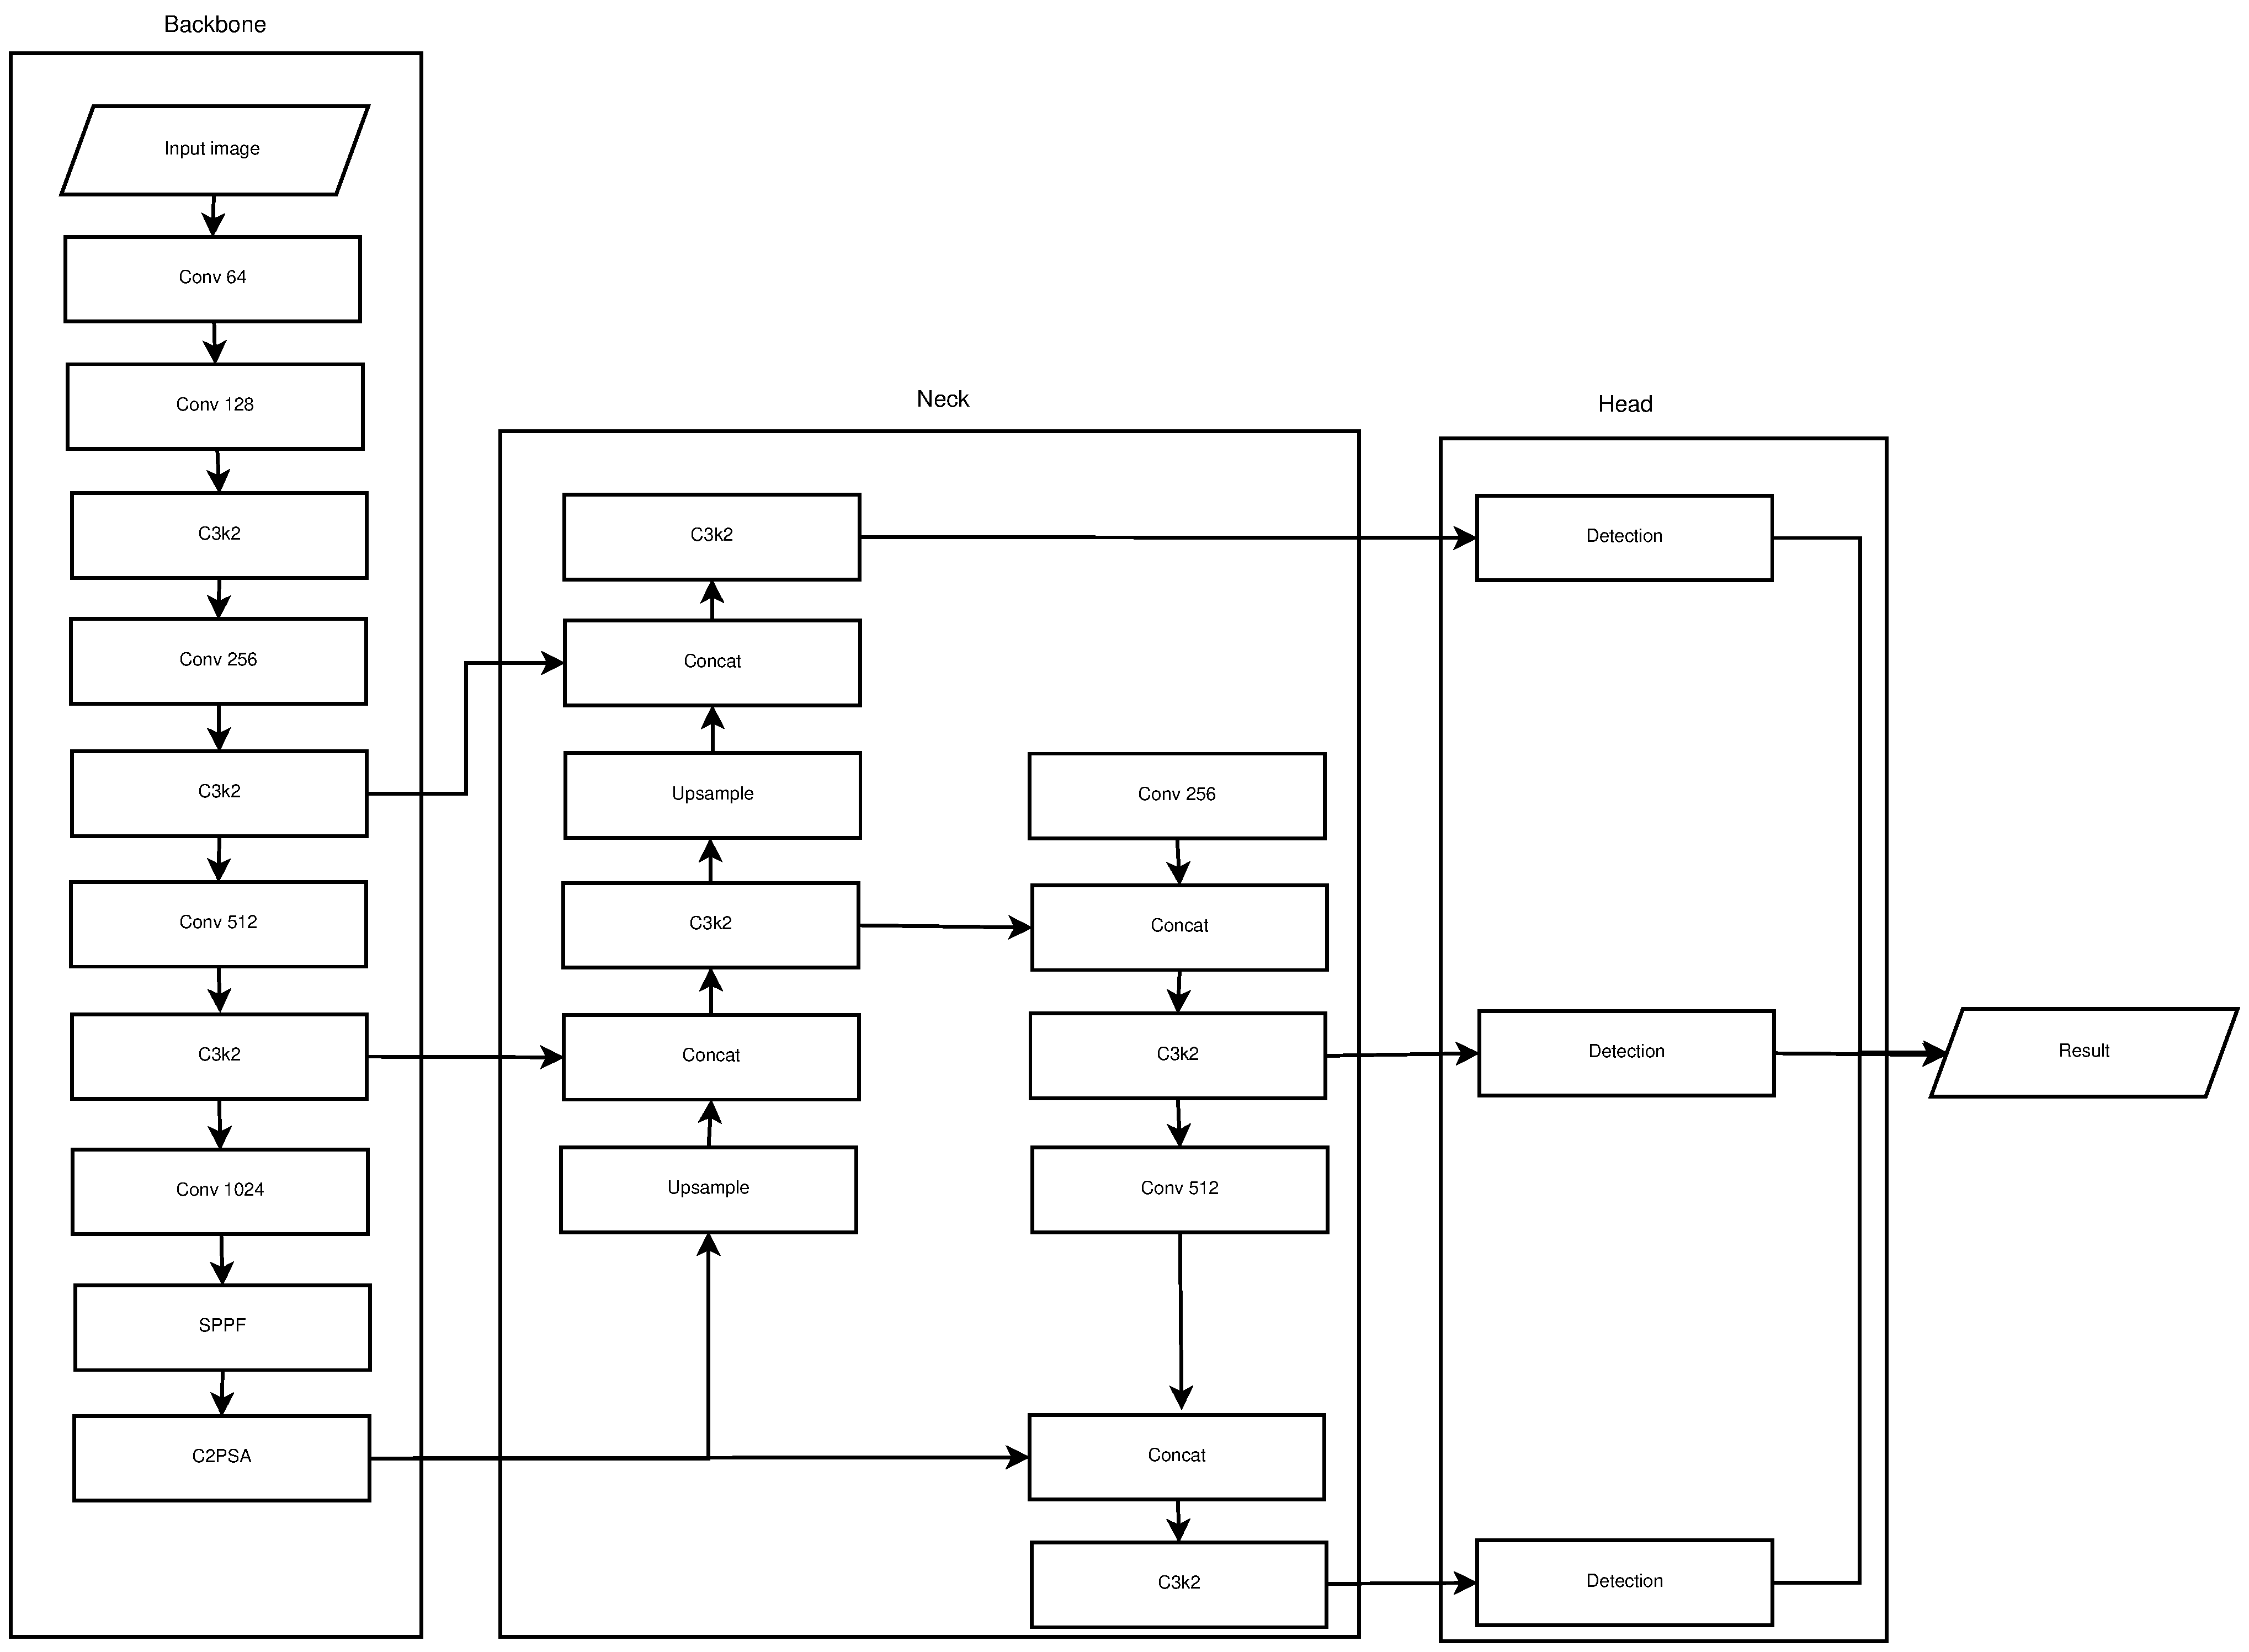
\includegraphics[width=1.05\linewidth, height=0.65\linewidth]{Yolo.eps}
		\caption{Архитектура YOLO 11}
		\label{йоло:image}
	\end{figure}
\end{landscape}
\paragraph{Backbone}

Backbone анализирует входное изображение размером 640x640 пикселей. Основной его задачей является выделение важных деталей, таких как края, текстуры или пятна на листе, которые характерны для заболеваний. Архитектура Backbone постепенно уменьшает размер изображения и увеличивает глубину признаков через следующие слои \cite{yolo8}:

\begin{enumerate}
	\item Conv 64 -- свёрточный слой с 64 фильтрами размером 3x3 и шагом 2, он уменьшает изображение с 640x640x3 до 320x320x64. При свёртке идёт обобщение крупных структур, таких как контуры листьев.
	
	\item Conv 128 -- свёрточный слой с 128 фильтрами размером 3x3 и шагом 2 уменьшает размер до 160x160x128, усиливая выделение текстурных особенностей.
	
	\item C3k2 -- улучшенный блок C3 с двумя свёрточными слоями и остаточными связями, которые пропускают часть входных данных через блок без изменений и добавляют их к выходу. Это предотвращает проблему затухающего градиента во время обратного распространения. На выходе имеем изображение 160x160x256.
	
	\item Conv 256 уменьшает размер до 80x80x256, фокусируясь на признаках средней детализации, таких как пятна 10–20 пикселей.
	
	\item Блок C3k2 с двумя свёрточными слоями преобразует данные до 80x80x512, выделяя более сложные текстуры, такие как пятна или повреждения листьев.
	
	\item Слой conv 512 формирует карту размером 40x40x512, фокусируется на объектах среднего размера.
	
	\item Блок C3k2 сохраняет размер 40x40x512, углубляет признаки.
	
	\item Conv 1024 формирует карту размером 20x20x1024, выделяет крупные области поражения.
	
	\item Блок C3k2 сохраняет размер 20x20x1024, углубляет признаки.
	
	\item SPPF применяет пулинг с разными масштабами ядер (5x5, 9x9, 13x13), чтобы захватить признаки разной детализации. В отличие от других методов пулинга, SPPF ускоряет этот процесс за счёт оптимизированных свёрток.
	 
	\item C2PSA основан на механизме само-внимания, который оценивает взаимосвязи между разными частями изображения. Это помогает модели сосредотачиваться на важных областях, таких как мелкие пятна или изменения цвета, игнорируя фоновые элементы.
	
\end{enumerate}

Backbone формирует карты признаков 80x80x256, 40x40x512, 20x20x1024 и передаёт  в neck.

\paragraph{Neck}

Neck собирает данные из backbone и готовит их к финальному этапу детекции. Эта часть объединяет информацию с разными масштабами, чтобы модель могла лучше находить мелкие объекты. Neck состоит из следующих модулей \cite{yolo3}:

\begin{enumerate}
	\item Слой Upsample преобразует 20x20x1024 в 40x40x1024, используя интерполяцию, что улучшает анализ мелких деталей.
	
	\item Слой Concat соединяет 40x40x1024 с 40x40x512, формируя 40x40x1536. Это помогает сделать карту признаков полнее.  

	\item Блок C3k2 преобразует 40x40x1536 в 40x40x512, углубляет признаки.
	
	\item Upsample преобразует 40x40x512 в 80x80x512, что улучшает анализ мелких объектов.
	
	\item Слой Concat формирует 80x80x768, соединяя 80x80x512 с 80x80x256.
	
	\item C3k2 выдаёт 80x80x256, углубляет признаки.
	
	\item Слой Conv 256 преобразует 80x80x256 в 40x40x256 и подготавливает данные для следующего масштаба.
	
	\item Concat соединяет 40x40x256 с 40x40x512 и формирует 40x40x768.
	
	\item Блок C3k2 выдаёт 40x40x512, углубляет признаки.
	
	\item Conv 512 преобразует 40x40x512 в 20x20x512.
	
	\item Concat формирует 20x20x1536, соединяя 20x20x512 с 20x20x1024. 
	
	\item C3k2 выдаёт 20x20x1024, углубляет признаки.

\end{enumerate}

Neck готовит три карты признаков размерностями 80x80x256, 40x40x512 и 20x20x1024 и отправляет их в head для диагностики.

\paragraph{Head}

Head -- это последняя часть модели, которая выдаёт результаты на основе данных из neck. Блок Detect обрабатывает каждый масштаб и делает предсказания координат рамок, вероятностей классов и уверенности. Он использует свёртки, чтобы получить эти данные.

\subsection{Структура модулей программы}

Программа для диагностики заболеваний томатов представляет собой веб-приложение, реализованное с использованием Python, модели YOLO11 для обнаружения болезней, PostgreSQL для хранения данных и HTML/CSS для клиентского интерфейса. Структура программы организована в виде набора модулей, каждый из которых выполняет определённые функции. На схеме ~\ref{модули:image} представлена структура разрабатываемого решения.
	\begin{figure}[H]
		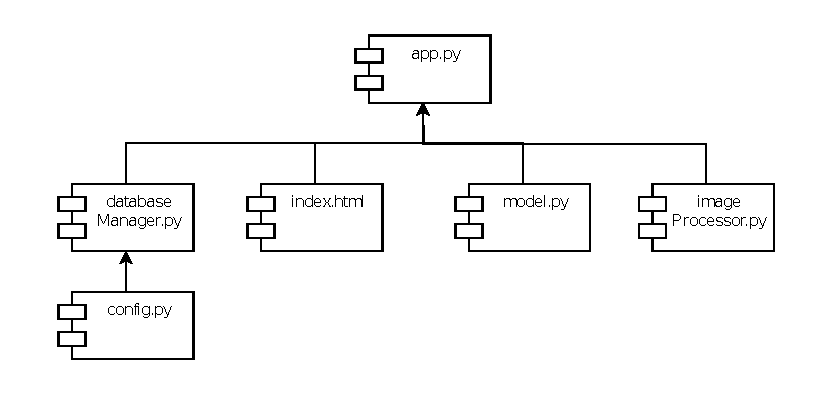
\includegraphics[width=1\linewidth]{Modules.eps}
		\caption{Структура модулей программы}
		\label{модули:image}
	\end{figure}

\begin{enumerate}
	\item Модуль app.py 
	Основной файл серверной части, реализованный на фреймворке Flask. Обрабатывает GET и POST запросы для загрузки изображений, кодирует изображения в base64 для отображения и запрашивает данные о болезни из базы данных.
	
	\item Модуль databaseManager.py
	Модуль для взаимодействия с базой данных PostgreSQL. Содержит класс Database для настройки соединения с базой, выполняет SQL-запросы для получения данных о болезни, включая методы лечения и профилактики.
	
	\item Модуль config.py
	Файл конфигурации, содержащий параметры подключения к базе данных.
	
	\item index.html
	HTML-шаблон клиентского интерфейса. Содержит форму для загрузки изображений, блок для отображения данных о болезни. Использует CSS-стили из файла styles.css.
	
	\item Модуль model.py. Загружает и настраивает обученную модель для анализ изображений и выявление заболеваний.
	
	\item Модуль imageProcessor.py. выполняет предварительную обработку изображений для анализа моделью и их преобразование для отображения в интерфейсе.
	
\end{enumerate}

\subsection{Структура базы данных}

Сущности и отношения между ними отображены на ER-диаграмме.

 \begin{figure}[ht]
	\center{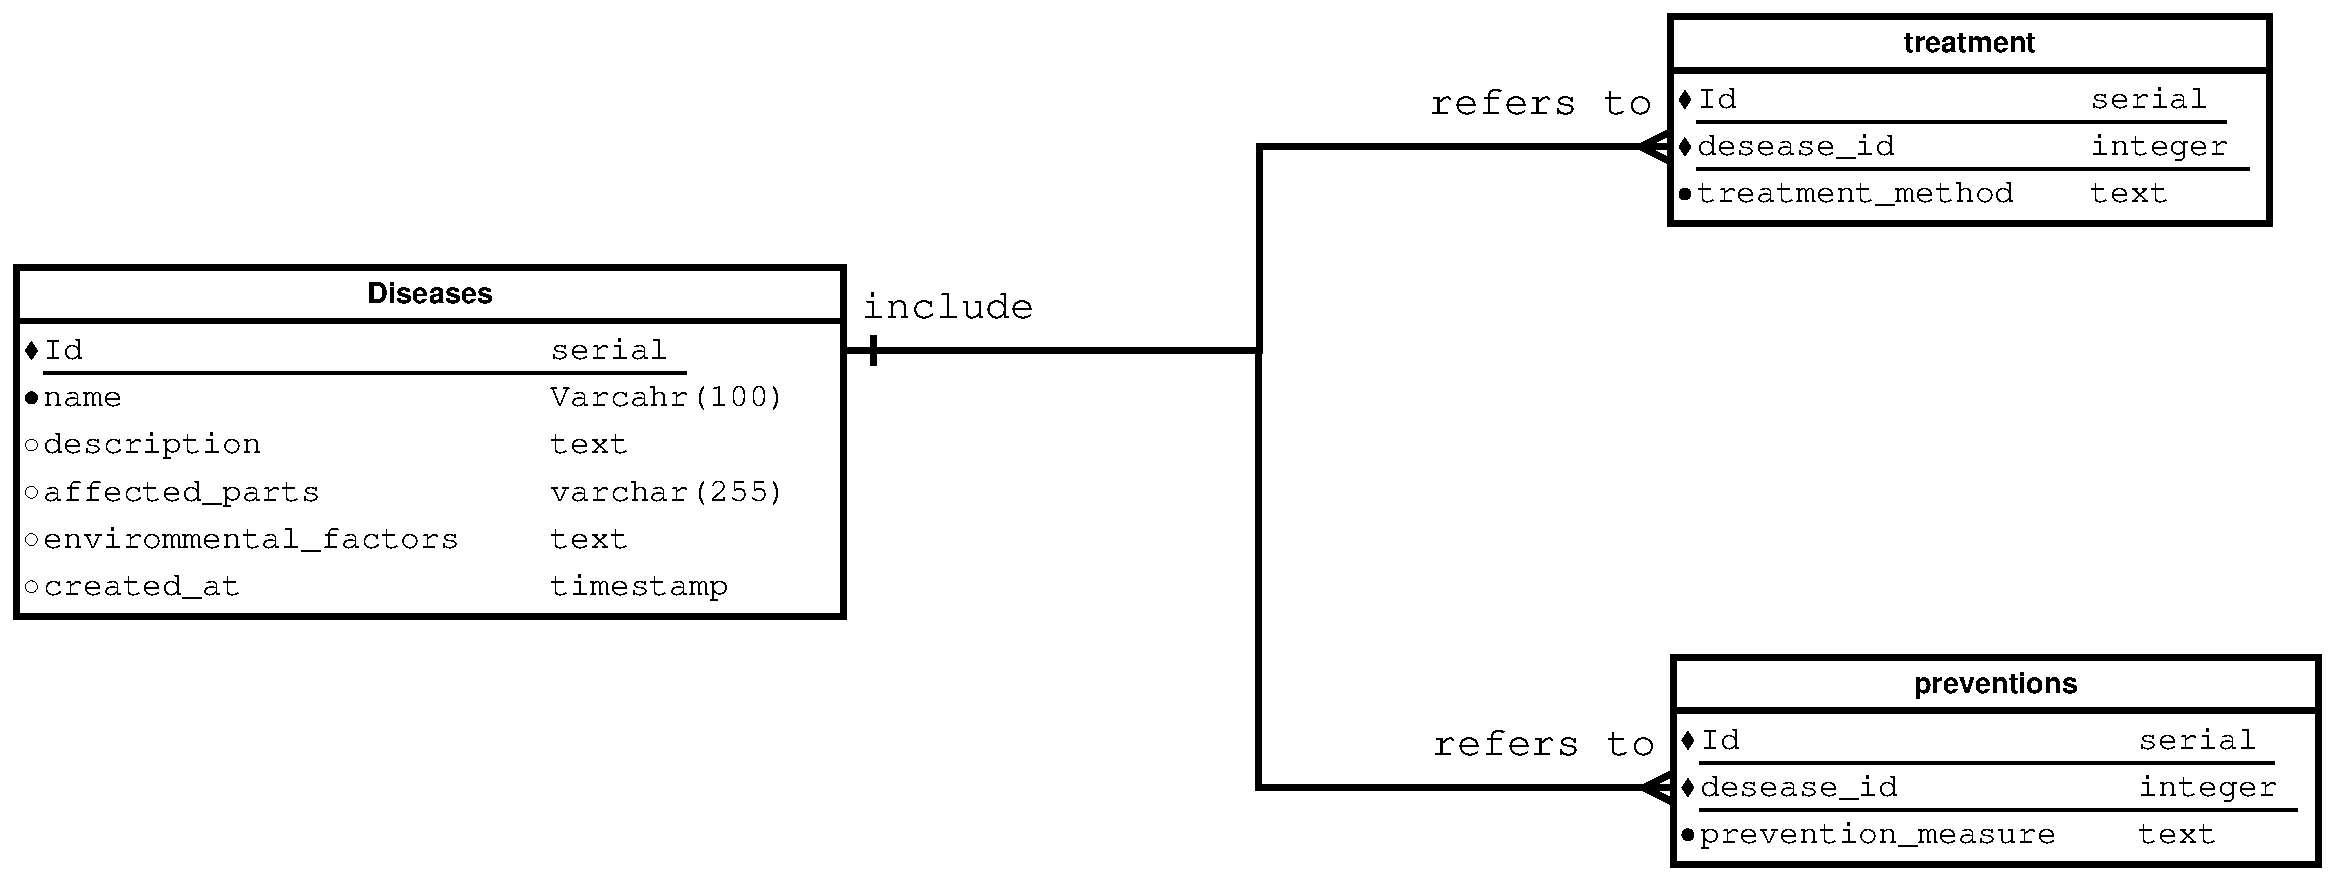
\includegraphics[width=1\linewidth, height=0.5\linewidth]{ДиаграммаБд}}
	\caption{ER-диаграмма}
	\label{er:image}
\end{figure}


\begin{xltabular}{\textwidth}{|l|l|p{1.7cm}|X|}
	\caption{Атрибуты сущности diseases\label{diseases:table}}\\ \hline
	\centrow Поле & \centrow Тип & \centrow Обяза\-тельное & \centrow Описание \\ \hline
	\thead{1} & \thead{2} & \centrow 3 & \centrow 4 \\ \hline
	\endfirsthead
	\caption*{Продолжение таблицы \ref{diseases:table}} \\ \hline
	\thead{1} & \thead{2} & \centrow 3 & \centrow 4 \\ \hline
	\finishhead
	id & serial & true & Первичный ключт \\ \hline
	name & varchar(100) & true & Название болезни \\ \hline
	description & text & false & Подробное описание болезни \\ \hline
	affected\_parts & varchar(255) & false & Части растения, поражаемые болезнью \\ \hline
	environmental\_factors & text & false & Экологические факторы, способствующие болезни \\ \hline
	created\_at & timestamp & false & Дата и время создания записи \\ \hline
\end{xltabular}

\begin{xltabular}{\textwidth}{|l|l|p{1.7cm}|X|}
	\caption{Атрибуты сущности treatments\label{treatments:table}}\\ \hline
	\centrow Поле & \centrow Тип & \centrow Обяза\-тельное & \centrow Описание \\ \hline
	\thead{1} & \thead{2} & \centrow 3 & \centrow 4 \\ \hline
	\endfirsthead
	\caption*{Продолжение таблицы \ref{treatments:table}} \\ \hline
	\thead{1} & \thead{2} & \centrow 3 & \centrow 4 \\ \hline
	\finishhead
	id & serial & true & Первичный ключ \\ \hline
	disease\_id & integer & true & Внешний ключ, ссылка на таблицу diseases \\ \hline
	treatment\_method & text & true & Описание методов лечения \\ \hline
\end{xltabular}

\begin{xltabular}{\textwidth}{|l|l|p{1.7cm}|X|}
	\caption{Атрибуты сущности preventions\label{preventions:table}}\\ \hline
	\centrow Поле & \centrow Тип & \centrow Обяза\-тельное & \centrow Описание \\ \hline
	\thead{1} & \thead{2} & \centrow 3 & \centrow 4 \\ \hline
	\endfirsthead
	\caption*{Продолжение таблицы \ref{preventions:table}} \\ \hline
	\thead{1} & \thead{2} & \centrow 3 & \centrow 4 \\ \hline
	\finishhead
	id & serial & true & Первичный ключ \\ \hline
	disease\_id & integer & true & Внешний ключ, ссылка на таблицу diseases \\ \hline
	prevention\_measure & text & true & Описание мер профилактики \\ \hline
\end{xltabular}

